% Kapitel 7
%-------------------------------------------------------------------------------


\chapter{Benutzeroberfläche}

Die Benutzeroberfläche wird unterteilt in mindestens drei Webseiten:
Ausgehend von einer Suchseite, werden die Ergebnisse tabellarisch unter der
Suchmaske angezeigt, die auf Detailseiten weiterführen. 
Der Benutzer hat je nach Rechtestatus eine Gast-/Benutzer- oder eine Administrationsumgebung (zum Beispiel zum normalen Einsehen, Verändern, Löschen von Komponenten). 

\section{/B10/ Seitenlayout}

 \begin{itemize}
   \item Komponentendatenbank
   \begin{itemize}
    \item Suche
      \begin{description}
       \item[Einfache Suche] Die einfache Suche soll relativ unkompliziert funktionieren:
        Sie besteht lediglich aus einer Eingabefläche, worin der Benutzer
       den Namen der Komponente, Autoren oder Sonstiges eingeben kann. 
       \item[Erweiterte Suche] Die erweiterte Suche stellt mehrere Optionen zur Verfügung, um die Suche zu präzisieren. 
       \end{description}
    \end{itemize}
    \item Verzeichnis
      \begin{description}
        \item[] Hier findet der Benutzer eine Liste von den verfügbaren Interfaces und ihren zugehörigen Komponenten.
        Durch Auswählen einer bestimmten Komponente, wird der Benutzer zu ihrer Detailseite weitergeleitet.
        Dort findet er neben der Beschreibung eine Übersicht zu den verantwortlichen Programmieren, der Versionsnummer, das Erstelldatum und auf welchem Server sich die betrachtete Komponente befindet. 
        Dem Benutzer wird zudem ein Link angeboten, um die gewünschte Komponente bei sich zu integrieren. 
      \end{description} 

    \item Anmeldung/Registrierung
      \begin{description}
        \item[Login] Der Benutzer kann sich mit seinem Benutzernamen/Passwort anmelden. Sollte er sein Passwort vergessen haben, gibt die Seite ihm per Eingabe seiner Mailadresse die Gelegenheit, sich ein Neues setzen zu lassen.
        \item[Registrieren]Der Benutzer kann sich mit einem beliebigen Benutzernamen und Passwort registrieren, die eine Emailadresse erfordert.
      \end{description}   
    
    \item Administration
 \end{itemize}
 
\begin{figure}
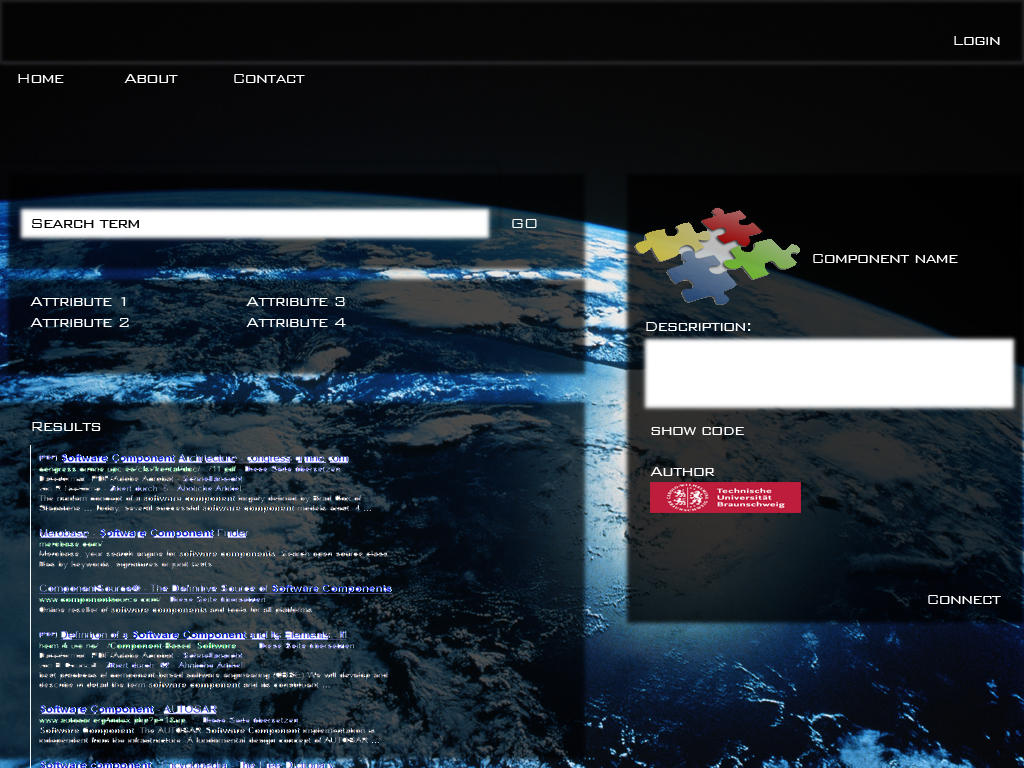
\includegraphics[width=0.8\linewidth]{bilder/overview.jpg}
\caption{Beispiel für ein Seitenlayout}
\label{fig:gui}
\end{figure}

Suchergebnisse werden in einem großen Bereich rechts bzw.\ unter der Navigation angezeigt. 
Die Komponenten werden übersichtlich in tabellenartiger Form bereitgestellt. Bei einem Klick auf ein bestimmtes Suchergebnisses erscheinen genauere Informationen über die Komponente. 
Oben rechts wird zudem der eingeloggte User angezeigt.
Bei einem Klick auf den eingeloggten User ist eine Account-Verwaltungsseite geplant.
